\chapter{Ergebnisse}

Sofern nicht anders erwähnt wurden Systeme mit zwei Intel Xeon Gold 6230 Prozessoren mit einer Taktrate von 2.1 Ghz und 180GB RAM benutzt.
Die Ergebnisse wurden auf gleichen System, aber nicht auf demselben erzeugt.

\section{Untersuchung der Graphen}

Die bereitgestellten Graphen wurden vor ihrer Nutzung untersucht
Hierfür wurde zuerst die Verteilung der Knotengrade untersucht.
Dabei wurden die Histogramme in \autoref{ergebnisse:fig:degree_hist} erstellt.
Für jeden der Sichtbarkeitsgraphen gilt, dass mindestens 90\% aller Knoten einen Grad kleiner \num{2000} haben.

\begin{figure}[p]
  \begin{subfigure}[b]{0.5\textwidth}
    \resizebox{\textwidth}{!}{%
      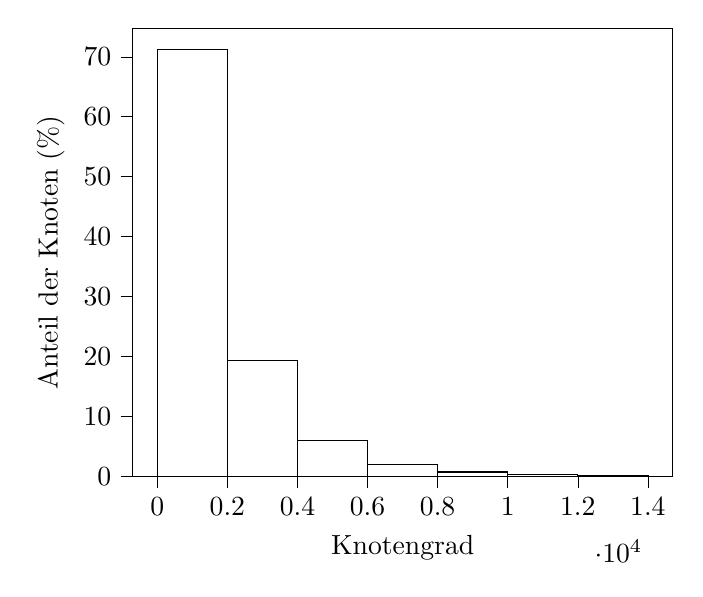
\begin{tikzpicture}
        \begin{axis}[
            tick align=outside,
            tick pos=left,
            xmin=-698, xmax=14702,
            xtick style={color=black},
            xtick distance=2000,
            ymin=0, ymax=0.747618384401001,
            ytick style={color=black},
            ytick={0,0.1,0.2,0.3,0.4,0.5,0.6,0.7,0.8},
            yticklabels={0,10,20,30,40,50,60,70,80},
            xlabel={Knotengrad},
            ylabel={Anteil der Knoten (\%)}
          ]
          \draw[] (axis cs:2,0) rectangle (axis cs:2002,0.712017508953334);
          \draw[] (axis cs:2002,0) rectangle (axis cs:4002,0.194220055711032);
          \draw[] (axis cs:4002,0) rectangle (axis cs:6002,0.0606247512935969);
          \draw[] (axis cs:6002,0) rectangle (axis cs:8002,0.0205382013530728);
          \draw[] (axis cs:8002,0) rectangle (axis cs:10002,0.00766514126545947);
          \draw[] (axis cs:10002,0) rectangle (axis cs:12002,0.00397930760049903);
          \draw[] (axis cs:12002,0) rectangle (axis cs:14002,0.000955033824119655);
        \end{axis}
      \end{tikzpicture}
    }
    \caption{aegaeis-vis}
  \end{subfigure}%
  \begin{subfigure}[b]{0.5\textwidth}
    \resizebox{\textwidth}{!}{%
      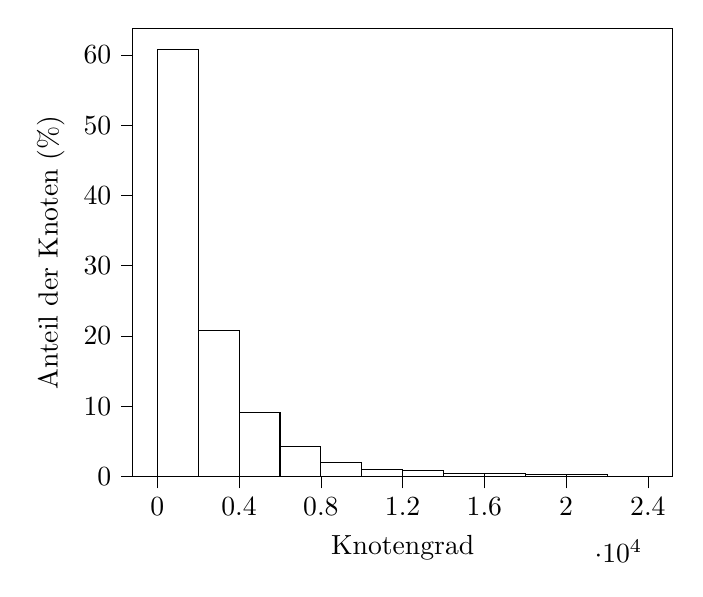
\begin{tikzpicture}
        \begin{axis}[
            tick align=outside,
            tick pos=left,
            xlabel={Knotengrad},
            xmin=-1198, xmax=25202,
            xtick distance=4000,
            xtick style={color=black},
            ylabel={Anteil der Knoten (\%)},
            ymin=0, ymax=0.637890337808629,
            ytick style={color=black},
            ytick={0,0.1,0.2,0.3,0.4,0.5,0.6,0.7},
            yticklabels={0,10,20,30,40,50,60,70}
          ]
          \draw[] (axis cs:2,0) rectangle (axis cs:2002,0.60751460743679);
          \draw[] (axis cs:2002,0) rectangle (axis cs:4002,0.207212784893063);
          \draw[] (axis cs:4002,0) rectangle (axis cs:6002,0.0905080679486225);
          \draw[] (axis cs:6002,0) rectangle (axis cs:8002,0.0423164235317719);
          \draw[] (axis cs:8002,0) rectangle (axis cs:10002,0.0196700589456533);
          \draw[] (axis cs:10002,0) rectangle (axis cs:12002,0.0103219440467273);
          \draw[] (axis cs:12002,0) rectangle (axis cs:14002,0.00818403436132265);
          \draw[] (axis cs:14002,0) rectangle (axis cs:16002,0.00425647177184629);
          \draw[] (axis cs:16002,0) rectangle (axis cs:18002,0.00420165357478464);
          \draw[] (axis cs:18002,0) rectangle (axis cs:20002,0.00342452501643997);
          \draw[] (axis cs:20002,0) rectangle (axis cs:22002,0.00236363167330556);
          \draw[] (axis cs:22002,0) rectangle (axis cs:24002,2.57967986172503e-05);
        \end{axis}
      \end{tikzpicture}
    }
    \caption{medi-vis}
  \end{subfigure}
  \par\bigskip
  \begin{subfigure}[b]{0.5\textwidth}
    \resizebox{\textwidth}{!}{%
      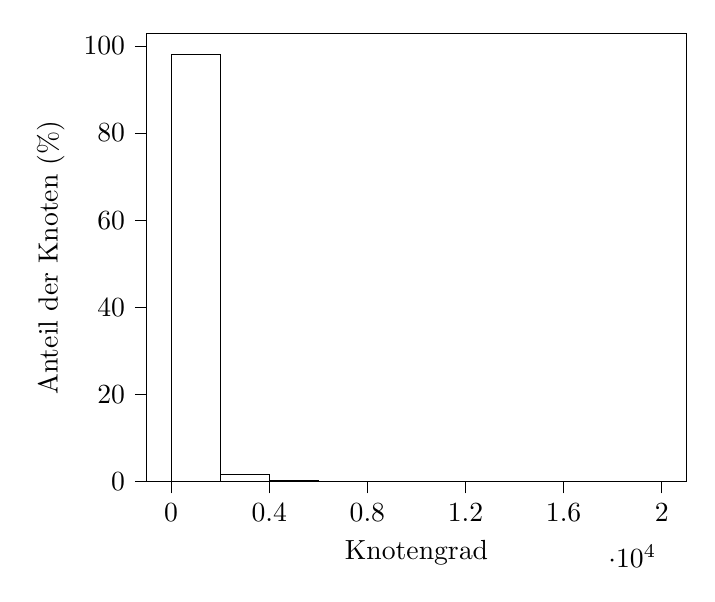
\begin{tikzpicture}
        \begin{axis}[
            tick align=outside,
            tick pos=left,
            xlabel={Knotengrad},
            ylabel={Anteil der Knoten (\%)},
            xmin=-998, xmax=21002,
            xtick style={color=black},
            y grid style={darkgray176},
            xtick distance=4000,
            ymin=0, ymax=1.02857224104146,
            ytick style={color=black},
            ytick={0,0.2,0.4,0.6,0.8,1,1.2},
            yticklabels={0,20,40,60,80,100,120}
          ]
          \draw[] (axis cs:2,0) rectangle (axis cs:2002,0.979592610515676);
          \draw[] (axis cs:2002,0) rectangle (axis cs:4002,0.0169022235303201);
          \draw[] (axis cs:4002,0) rectangle (axis cs:6002,0.00222602483448042);
          \draw[] (axis cs:6002,0) rectangle (axis cs:8002,0.000968834654540784);
          \draw[] (axis cs:8002,0) rectangle (axis cs:10002,0.000297335455255565);
          \draw[] (axis cs:10002,0) rectangle (axis cs:12002,3.99107993631631e-06);
          \draw[] (axis cs:12002,0) rectangle (axis cs:14002,0);
          \draw[] (axis cs:14002,0) rectangle (axis cs:16002,9.97769984079078e-07);
          \draw[] (axis cs:16002,0) rectangle (axis cs:18002,3.99107993642733e-06);
          \draw[] (axis cs:18002,0) rectangle (axis cs:20002,3.99107993631631e-06);
        \end{axis}

      \end{tikzpicture}
    }
    \caption{pata-vis}
  \end{subfigure}
  \caption{Verteilung der Kantengrade}
  \label{ergebnisse:fig:degree_hist}
\end{figure}

Wie diskutiert ist die Summe der quadratischen Knotengrade ein Indikator für die Performanz der Kontraktion.
Diese sind in \autoref{table:sum_quad_degree} sichtbar.
Obwohl pata die meisten Knoten hat, ist die summe der Quadrate am kleinsten.

Dann naive Rechnung: Knoten-Differenz soll in einem Tag stattfinden, 40 Kerne.
Wieviel Zeit pro Paar?

\begin{table}[ht]
  \centering
  \begin{tabular}{
      l % Graph
      S[table-format = 13.0] % Zeit
      S[table-format = 3.1] % Zeit pro Paars
    }
    \toprule
    {Graph}            & {$\sum_{v \in V} (\text{Grad}(v))^2$} & {Zeit pro paar in us}                       \\ \midrule
    aegaeis-visibility & 1153579966074                         & \fpeval{(10e6)*40*(24*60*60)/1153579966074} \\
    medi-visibility    & 4667069733248                         & \fpeval{(10e6)*40*(24*60*60)/4667069733248} \\
    pata-visibility    & 426189267238                          & \fpeval{(10e6)*40*(24*60*60)/426189267238}  \\ \bottomrule
  \end{tabular}
  \caption{Summe quadratische Knotengrade}
  \label{table:sum_quad_degree}
\end{table}

\begin{figure}[p]% Die Daten in den .csv Dateien sind gelippt auf 100. pgf hat Probleme mit zu großen Zahlen.
  \begin{subfigure}[b]{0.5\textwidth}
    \resizebox{\textwidth}{!}{%
      \begin{tikzpicture}
        \begin{axis}[
            ymax=6,
            xlabel={Hop-Länge},
            ylabel={Fehler (\%)},
            legend style={at={(1,0.475)},anchor=east, nodes={scale=0.8, transform shape}}
          ]
          \addplot+[mark repeat=9] table [x=hops, y=simple_graph_upper_bound, col sep=comma] {data/bounds/aegaeis.csv};
          \addlegendentry{$\triangle$};

          \addplot+[mark repeat=9] table [x=hops, y=10, col sep=comma] {data/bounds/aegaeis.csv};
          \addlegendentry{10 Hubs};

          \addplot+[mark repeat=9] table [x=hops, y=20, col sep=comma] {data/bounds/aegaeis.csv};
          \addlegendentry{20 Hubs};

          \addplot+[mark repeat=9] table [x=hops, y=40, col sep=comma] {data/bounds/aegaeis.csv};
          \addlegendentry{40 Hubs};

          \addplot+[mark repeat=9] table [x=hops, y=80, col sep=comma] {data/bounds/aegaeis.csv};
          \addlegendentry{80 Hubs};

          \addplot+[mark repeat=9] table [x=hops, y=min_80_simple, col sep=comma] {data/bounds/aegaeis.csv};
          \addlegendentry{$\triangle$, 80 Hubs};
        \end{axis}
      \end{tikzpicture}
    }
    \caption{aegaeis-vis}
  \end{subfigure}%
  \begin{subfigure}[b]{0.5\textwidth}
    \resizebox{\textwidth}{!}{%
      \begin{tikzpicture}
        \begin{axis}[
            ymax=6,
            xlabel={Hop-Länge},
            ylabel={Fehler (\%)},
            legend style={at={(1,0.475)},anchor=east, nodes={scale=0.8, transform shape}}
          ]
          \addplot+[mark repeat=12] table [x=hops, y=simple_graph_upper_bound, col sep=comma] {data/bounds/medi.csv};
          \addlegendentry{$\triangle$};

          \addplot+[mark repeat=12] table [x=hops, y=10, col sep=comma] {data/bounds/medi.csv};
          \addlegendentry{10 Hubs};

          \addplot+[mark repeat=12] table [x=hops, y=20, col sep=comma] {data/bounds/medi.csv};
          \addlegendentry{20 Hubs};

          \addplot+[mark repeat=12] table [x=hops, y=40, col sep=comma] {data/bounds/medi.csv};
          \addlegendentry{40 Hubs};

          \addplot+[mark repeat=12] table [x=hops, y=80, col sep=comma] {data/bounds/medi.csv};
          \addlegendentry{80 Hubs};

          \addplot+[mark repeat=12] table [x=hops, y=min_80_simple, col sep=comma] {data/bounds/medi.csv};
          \addlegendentry{$\triangle$, 80 Hubs};
        \end{axis}
      \end{tikzpicture}
    }
    \caption{medi-vis}
  \end{subfigure}
  \par\bigskip
  \begin{subfigure}[b]{0.5\textwidth}
    \resizebox{\textwidth}{!}{%
      \begin{tikzpicture}
        \begin{axis}[
            ymax=6,
            xlabel={Hop-Länge},
            ylabel={Fehler (\%)},
            legend style={at={(1,0.475)},anchor=east, nodes={scale=0.8, transform shape}}
          ]
          \addplot+[mark repeat=25] table [x=hops, y=simple_graph_upper_bound, col sep=comma] {data/bounds/pata.csv};
          \addlegendentry{$\triangle$};

          \addplot+[mark repeat=25] table [x=hops, y=10, col sep=comma] {data/bounds/pata.csv};
          \addlegendentry{10 Hubs};

          \addplot+[mark repeat=25] table [x=hops, y=20, col sep=comma] {data/bounds/pata.csv};
          \addlegendentry{20 Hubs};

          \addplot+[mark repeat=25] table [x=hops, y=40, col sep=comma] {data/bounds/pata.csv};
          \addlegendentry{40 Hubs};

          \addplot+[mark repeat=25] table [x=hops, y=80, col sep=comma] {data/bounds/pata.csv};
          \addlegendentry{80 Hubs};

          \addplot+[mark repeat=25] table [x=hops, y=min_80_simple, col sep=comma] {data/bounds/pata.csv};
          \addlegendentry{$\triangle$, 80 Hubs};
        \end{axis}
      \end{tikzpicture}
    }
    \caption{pata}
  \end{subfigure}
  \caption{Fehler der oberen Schranken}
\end{figure}

\todo{Boxplot für alle Hops über 80 und Triangulierung}

% aegaeis
% 75.6658\% korrekt
% 0.40990444596118253 average
%
% %WARUM MEDI, PATA nicht so korrekt?
% \todo{STIMMEN ZAHLEN?}
%
% medi
% 0.39110000000000006\% korrekt
% 0.9727677753480117 average
%
% pata
% 0.068\% korrekt
% 0.6179520250326755 average

\section{Dijkstra}

Für die Berechnung des Speedups der in dieser Arbeit angewandeten Methoden wurden für jeden Graph \num{1000} sequentielle $s$-$t$ Dijkstra-Suchen asugeführt und die durschnittliche Laufzeit ermittelt.
Die durschnittliche Laufzeiten für das Finden und erstellen des kürzesten Pfad sind in Tabelle \ref{fig:ergebnisse:dijkstra} dargestellt.
Es ist ersichtlich, dass die Sichtbarkeitsgraphen im Vergleich zu ihren Triangulierungen deutlich höhere Laufzeiten haben.

Zusätzlich zur durschnitlichen Laufzeit wurde die die Durschnitswerte der Hop-Länge, des Dijsktra-Rank und der Queue pops ermittelt, um ein Verständnis für die Laufzeiten zu erlangen.
Es zeigte sich, dass die durschnittliche Hop-Länge der Sichtbarkeitsgraphen deutlich signifikant kürzer ist, als die der Triangulierungen.
Obwohl die Sichtbarkeitsgraphen eine niedriger Anzahl an Knoten haben, ist die durschnitliche Anzahl der Queue pops größer.
Dies legt Nahe, dass die verwendung einer Warteschlange, welche eine \emph{Drecrease-Key} Funktion anbietet, die Geschwindigkeit der Dijkstra Suche erhöhen würde.

\begin{table}[h!]
  \centering
  \begin{tabular}{
      l % Graph
      S[table-format = 4.1] % Zeit
      S[table-format = 3.0] % hop-länge
      S[table-format = 7.0] % rank
      S[table-format = 7.0] % queue pops
    }
    \toprule
    {Graph}            & {$\varnothing$ $t({spd})$} & {$\varnothing$  Hop-Länge} & {$\varnothing$ Dijkstra Rank} & {$\varnothing$ Queue pops} \\
                       & {(\si{\ms})}               &                            &                               &                            \\
    \midrule
    aegaeis-graph      & 60.281198                  & 215.7201                   & 260447.36                     & 325845.56                  \\
    aegaeis-visibility & 630.434928                 & 16.311                     & 98650.82                      & 517346.63                  \\
    medi-graph         & 87.08376                   & 340.445                    & 394855.78                     & 494553.97                  \\
    medi-visibility    & 1279.67479                 & 23.6149                    & 154092.42                     & 959206.4                   \\
    pata-graph         & 265.825771                 & 883.979                    & 1120841.9                     & 1387047.8                  \\
    pata-visibility    & 1017.695977                & 63.817                     & 498570.2                      & 2429689.8                  \\ \bottomrule
  \end{tabular}
  \caption{Durschnitliche Kennwerte der Dijkstra Suchen (über \num{10000} Suchen)}
  \label{fig:ergebnisse:dijkstra}
\end{table}

\section{Graphen-Kontraktion}

Ausgangspunkt der Analyzse, ob sich die in dieser Arbeit bearbeiteten Sichtbarkeitsgraphen kontrahieren lassen, war die Anwendung der klassischen Graphen-Kontraktion mit Witness-Suche, wobei ein für diese Arbeit entwickeltes Programm genutzt wurde.
Die Reihenfolge der Kontrraktion wurde dabei durch die Kanten-Differenz mit Lazy-Popping bestimmt.
Für die triangulierten Graphen war es möglich einen Contracted-Graphen zu erstellen, die Bearbeitung der Sichtbarkeitsgraphen wurde nach drei Tagen abgebrochen, wobei in dieser Zeit noch nicht alle initalen Kanten-Differenzen berechnet wurden.
Die Ergebnisse der trianguleirten Graphen sind in Tabelle \autoref{fig:ergebnisse:ch_graph_kontraktion_triangulierungen} zu sehen.

\begin{table}[h!]
  \centering
  \begin{tabular}{
      l % Graph
      r % Erstellung
      S[table-format = 1.2] % Abkürzungen/Katen
      S[table-format = 9.0] % average time spd
      S[table-format = 4.0] % speedup
    }
    \toprule
    {Graph}       & {Erstellung} & {$\frac{\text{Abkürzungen} (C)}{\text{Kanten} (G)}$} & {$\varnothing$ $t({spd})$} & {Speedup}                          \\
    {}            & {(min)}      & {}                                                   & {(\si{\us})}               & {}                                 \\
    \midrule
    aegaeis-graph & 2m 22s       & \fpeval{3047836/2795322}                             & 313.966                    & \fpeval{(60.281198*1000)/313.966}  \\
    medi-graph    & 3m 17s       & \fpeval{4535136/4223566}                             & 304.089                    & \fpeval{(87.08376*1000)/304.089}   \\
    pata-graph    & 9m 54s       & \fpeval{14187336/11632900}                           & 435.552                    & \fpeval{(265.825771*1000)/435.552} \\  \bottomrule
  \end{tabular}
  \caption{CH Graphen-Kontraktion}
  \label{fig:ergebnisse:ch_graph_kontraktion_triangulierungen}
\end{table}

Bassierend auf den Contracted-Graphen wurde jeweils ein Hub-Graph berechnet, die Ergebnisse hierfür sind in \autoref{fig:ergebnisse:hl_graph_kontraktion_triangulierungen} zu sehen.

\begin{table}[h!]
  \centering
  \begin{tabular}{
      l % Graph
      r % Erstellung
      S[table-format = 3.0] % label
      S[table-format = 3.2] % average time spd
      S[table-format = 6.] % speedup
    }
    \toprule
    {Graph}       & {Erstellung}     & {$\varnothing$ $\abs{\text{Label}}$} & {$\varnothing$ $t({spd})$} & {Speedup}                        \\
    {}            & {}               & {}                                   & {(\si{\us})}               & {}                               \\
    \midrule
    aegaeis-graph & 7m 11s           & 141.4722365640974                    & 2.334                      & \fpeval{(60.281198*1000)/2.334}  \\
    medi-graph    & 9m \phantom{0}1s & 115.88322360565405                   & 1.893                      & \fpeval{(87.08376*1000)/1.893}   \\
    pata-graph    & 29m 45s          & 133.48887779929734                   & 2.415                      & \fpeval{(265.825771*1000)/2.415} \\
    \bottomrule
  \end{tabular}
  \caption{HL Graphen-Kontraktion}
  \label{fig:ergebnisse:hl_graph_kontraktion_triangulierungen}
\end{table}

Als zusätzlicher Anhaltspunkt um die Qualität der erzeugten Contracted-Graphen zu beurteilen wurde ein externes Programm benutzt, um ebenfalls Contracted-Graphen zu erzeugen.
Die Ergebnisse hierfür sind in \autoref{fig:ergebnisse:fmi_ch_graph_kontraktion_triangulierungen} aufgelistet.
Da dieses Programm ein anders Format zur Speicherung benutz, wurden die Anfrage-Zeiten nicht erhoben.
Dieses Programm kontrahiert mehrere Knoten gleichzeitig, indem es \emph{Unabhänige Teilmengen} von Knoten findet, und kann daher besser parallel arbeiten, durch den hohen Grad der Sichtbarkeitsgraphen ist jedoch anzunehmen, dass es nur wenige, kleine unabhängige Teilmengen gibt.
Auch dieses Programm hat nach drei Tagen Laufzeit auf den Sichtbarkeitsgraphen keine Ergebnisse produziert.


\begin{table}[h!]
  \centering
  \begin{tabular}{
      l % Graph
      r % Erstellung
      S[table-format = 1.2] % Abkürzungen/Katen
      S[table-format = 9.0] % average time spd
      S[table-format = 4.0] % speedup
    }
    \toprule
    {Graph}       & {Erstellung} & {$\frac{\text{Abkürzungen} (C)}{\text{Kanten} (G)}$} \\
    {}            & {(min)}      & {}                                                   \\
    \midrule
    aegaeis-graph & 22s          & \fpeval{(5446922-(2795322/2))/2795322}               \\
    medi-graph    & 34s          & \fpeval{(8156314-(4223566/2))/4223566}               \\
    pata-graph    & 1m 48s       & \fpeval{(23557322-(11632900/2))/11632900}            \\  \bottomrule
  \end{tabular}
  \caption{FMI CH Graphen-Kontraktion}
  \label{fig:ergebnisse:fmi_ch_graph_kontraktion_triangulierungen}
\end{table}

\subsection{Kontraktion mit oberer Schranke}

\todo{Alles :D}

\section{PEOPLE}

Die in \autoref{chapter:peopel} vorgestellte Methode zur Berechnung von Contracted und Hub Graphen lies sie auch die Sichtbarkeitsgraphen und ihre Triangulierungen anwenden.

\subsection{Contracted Graph}

Die in \autoref{chapter:peopel} vorgestellte Methode zur Berechnung eines Contracted Graphens lies sich auf alle Graphen anwenden.
Die erzielten Werte der ERstellung sind in \autoref{table:ergebnisse:people_ch_erstellung} gesammelt.

Der Speedup ist in \autoref{table:ergebnisse:people_ch_speedup} zusammgenfasst.
Der Speedup der Trianuglierten Graphen ist deutlich kleiner, als der mit CH Witness, jedoch eine größenordnung schneller.
Der Speedup der Sichtbarkeitsgraphen ist kleines als eine Größenordnung.
Das sollte noch erkundet werden, warum.

pata hat trotzem mehr Speedup, weil von der Struktur her schon fast ein Straßengraph

\begin{table}[h!]
  \centering
  \begin{tabular}{
      l % Graph
      S[table-format = 4.0] % Erstellung
      S[table-format = 1.2] % Abkürzungen/Katen
      S[table-format = 3.2] % average time spd
      S[table-format = 3.2] % speedup
    }
    \toprule
    {Graph}            & {Erstellung} & {$\frac{\text{Abkürzungen} (C)}{\text{Kanten} (G)}$} & {$\varnothing$ $t({spd})$} & {Speedup}                      \\
    {}                 & {}           & {}                                                   & {(\si{\ms})}               & {}                             \\ \midrule
    aegaeis-graph      &              & \fpeval{12443056/2795322}                            & 2.290886                   & \fpeval{60.281198/2.290886}    \\
    aegaeis-visibility &              & \fpeval{214987558/310231834}                         & 408.948758                 & \fpeval{630.434928/408.948758} \\
    medi-graph         &              & \fpeval{20003908/4223566}                            & 3.38788                    & \fpeval{87.08376/3.38788}      \\
    medi-visibility    &              & \fpeval{468641256/730772544}                         & 832.555567                 & \fpeval{1279.67479/832.555567} \\
    pata-graph         &              & \fpeval{70624466/11632900}                           & 10.16729                   & \fpeval{265.825771/10.16729}   \\
    pata-visibility    &              & \fpeval{613324174/315653758}                         &                            & \fpeval{1017.695977/1}         \\  \bottomrule
  \end{tabular}
  \caption{Speedup der mit PEOPLE erstellten Contracted Graphen}
  \label{table:ergebnisse:people_ch_speedup}
\end{table}

\subsection{Hub Graph}

\subsubsection{Bootstraping HL}

Das Merging war deutlicht teruer als erwartet.
Dies ist dadurch zu erklären, dass für jeden Knoten die Anzahl der ausgehenden Contrated Graph Knoten viele Labels gemerged werden, welche durschnitlich sehr groß sind.
Das Mergen lässt sich aber gut parallisieren, durch eine Fold Operation, bei der jeder Thread für sich eine Menge an Labels merged.

\begin{table}[ht]
  \centering
  \begin{tabular}{ % DIREKT
      l % Graph
      S[table-format = 4.0] % creation zeit
      S[table-format = 4.1] % average time
    }
    \toprule
    {Graph}            & {Erstellung}       & {$\varnothing$ Label Größe} \\
    {}                 & {(min)}            & {}                          \\ \midrule
    aegaeis-graph      & 86.55              & 225.21998319619112          \\
    aegaeis-visibility & 357.9166666666667  & 2447.866444488659           \\
    medi-graph         & 191.06666666666666 & 262.34248736183486          \\
    medi-visibility    & 1317.85            & 3528.6126965393596          \\
    pata-graph         & 1706.5333333333333 & 451.8001829187458           \\
    pata-visibility    & 2657.5             & 1823.062327697596           \\  \bottomrule
  \end{tabular}
  \caption{Erstellung von Hub Graphen mit PEOPLE}
\end{table}


\begin{table}[h!]
  \centering
  \begin{tabular}{
      l % Graph
      r % Erstellung
      S[table-format = 3.0] % label
      S[table-format = 3.2] % average time spd
      S[table-format = 6.] % speedup
    }
    \toprule
    {Graph}       & {Erstellung}     & {$\varnothing$ $\abs{\text{Label}}$} & {$\varnothing$ $t({spd})$} & {Speedup}                        \\
    {}            & {}               & {}                                   & {(\si{\us})}               & {}                               \\
    \midrule
    aegaeis-graph & 7m 11s           & 141.4722365640974                    & 2.334                      & \fpeval{(60.281198*1000)/2.334}  \\
    medi-graph    & 9m \phantom{0}1s & 115.88322360565405                   & 1.893                      & \fpeval{(87.08376*1000)/1.893}   \\
    pata-graph    & 29m 45s          & 133.48887779929734                   & 2.415                      & \fpeval{(265.825771*1000)/2.415} \\
    \bottomrule
  \end{tabular}
  \caption{Erstellung von Hub Graphen mit PEOPLE}
\end{table}

\subsubsection{Direkt HL}

Das Anwenden des des Algorithmus zur Berechnung des Hub GRaphens hat gut funktioniert.
\todo{DIE LABELS SIND MINIMAL UNTERSCHIEDLICH GROß}

\begin{table}[ht]
  \centering
  \begin{tabular}{% MERGE ONLY
      l % Graph
      S[table-format = 4.0] % creation zeit
      S[table-format = 4.1] % average time
    }
    \toprule
    {Graph}            & {Erstellung}       & {$\varnothing$ Label Größe} \\
    {}                 & {(min)}            & {}                          \\ \midrule
    aegaeis-graph      & 12.3               & 225.18963155458096          \\
    aegaeis-visibility & 455.48333333333335 & 2446.9511241543973          \\
    medi-graph         & 19.75              & 262.32183266591755          \\
    medi-visibility    & 1338.4833333333333 & 3527.5645951837378          \\
    pata-graph         & 82.48333333333333  & 451.71017734369667          \\
    pata-visibility    & 847.2833333333333  & 1822.0561604813242          \\  \bottomrule
  \end{tabular}
  \caption{Erstellung von Hub Graphen durch Merging der mit PEOPLE erzeugen Contracted Graphen}
\end{table}

\subsubsection{Vergleich}

Für die Sichtbarkeitsgraphen ist es effizienter direkt die HL zu berechen.
Für die Triangulierten gRaphen ist es effizietner zuerst die  Contrated Graphen zu berechen.

\begin{table}[ht]
  \centering
  \begin{tabular}{ %VERGLEICH
      l % Graph
      S[table-format = 4.0] % creation zeit
      S[table-format = 4.0] % average time
    }
    \toprule
    {Graph}            & {CH \& Merging}               & {HL DIREKT}                  \\
    {}                 & {(min)}                       & {(min)}                      \\ \midrule
    aegaeis-graph      & \bfseries 32.5                & 86.55                        \\
    aegaeis-visibility & 809.3                         & \bfseries  357.9166666666667 \\
    medi-graph         & \bfseries  57.96666666666667  & 191.06666666666666           \\
    medi-visibility    & 2591.15                       & \bfseries  1317.85           \\
    pata-graph         & \bfseries  424.65000000000003 & 1706.5333333333333           \\
    pata-visibility    & 3532.366666666667             & \bfseries 2657.5             \\  \bottomrule
  \end{tabular}
  \caption{HL  merged}
\end{table}

\subsection{Vertex-to-level Vergeleich}

\begin{table}[]
  \centering
  \begin{tabular}{l
      S[table-format = 6.0] % random
      S[table-format = 6.0] % random
      S[table-format = 6.0] % random
      S[table-format = 6.0] % random
      S[table-format = 6.0] % random
      S[table-format = 6.0] % random
    }
    \toprule
    Graph              & \multicolumn{3}{c}{Hitting-Set}          & {$\triangle$}     & {Zufällig} & {Grad}   \\ \cline{2-4}
                       & {Zufällig} & {Hits}            & {Grad}  &                   &            &          \\
    \midrule
    aegaeis-visibility & 1747.03    & \bfseries 1420.17 & 1582.00 & 1473.27           & 17811.58   & 7420.85  \\
    medi-visibility    & 2487.06    & 2002.87           & 2422.12 & \bfseries 1930.65 & 18700.13   & 12862.80 \\
    pata-visibility    & 1100.42    & \bfseries 478.80  & 806.95  & 552.90            & 23690.52   & 10174.37 \\
    \bottomrule
  \end{tabular}
\end{table}